\documentclass[aspectratio=169,11pt]{beamer}
\usetheme{default}
\setbeamertemplate{navigation symbols}{}
\setbeamertemplate{footline}[frame number]

\usepackage{booktabs}
\usepackage{amsmath}
\usepackage{tikz}

%---------------------------------------------------------------------- colors
% navy  : titles and derived equations/results
% amber : assumptions
% green : numerical estimates
% red   : conclusions
\definecolor{navy}{HTML}{1F3A5F}
\definecolor{amber}{HTML}{C77700}
\definecolor{estc}{HTML}{1D7A6B}
\definecolor{alertc}{HTML}{B03A2E}

\setbeamercolor{frametitle}{fg=white,bg=navy}
\setbeamercolor{title}{fg=navy}
\setbeamercolor{subtitle}{fg=navy!70}
\setbeamercolor{structure}{fg=navy}
\setbeamercolor{alerted text}{fg=alertc}
\setbeamercolor{footline}{fg=navy!60}
\setbeamertemplate{frametitle}{%
  \nointerlineskip
  \begin{beamercolorbox}[wd=\paperwidth,ht=2.6ex,dp=1.1ex,leftskip=1em]{frametitle}
    \usebeamerfont{frametitle}\insertframetitle
  \end{beamercolorbox}\vspace{0.4em}}
\setbeamertemplate{blocks}[rounded][shadow=false]

\newenvironment{assume}[1]{%
  \setbeamercolor{block title}{fg=white,bg=amber}%
  \setbeamercolor{block body}{fg=black,bg=amber!9}%
  \begin{block}{#1}}{\end{block}}
\newenvironment{estimate}[1]{%
  \setbeamercolor{block title}{fg=white,bg=estc}%
  \setbeamercolor{block body}{fg=black,bg=estc!8}%
  \begin{block}{#1}}{\end{block}}
\newenvironment{result}[1]{%
  \setbeamercolor{block title}{fg=white,bg=navy}%
  \setbeamercolor{block body}{fg=black,bg=navy!7}%
  \begin{block}{#1}}{\end{block}}
\newcommand{\concl}[1]{{\color{alertc}\textbf{$\Rightarrow$ #1}}}

%---------------------------------------------------------------------- notation
\newcommand{\dd}{\mathrm{d}}
\newcommand{\Tch}{T_{\rm ch}}
\newcommand{\TTR}{T_{\rm TR}}
\newcommand{\LTR}{L_{\rm TR}}
\newcommand{\PTR}{P_{\rm TR}}
\newcommand{\qch}{q_{\rm ch}}
\newcommand{\kg}{\frac{2\gamma}{\gamma-1}}

\title{Pressure at the chromosphere top\\ from an analytic transition region}
\subtitle{Notation follows Sokolov et al.\ (2021)}
\author{Keheng Zhu}
\date{16 November 2026}

\begin{document}

\begin{frame}
  \titlepage
\end{frame}

%----------------------------------------------------------------------
\begin{frame}{Setup}
  \begin{columns}[T]
    \begin{column}{0.5\textwidth}
      \centering
      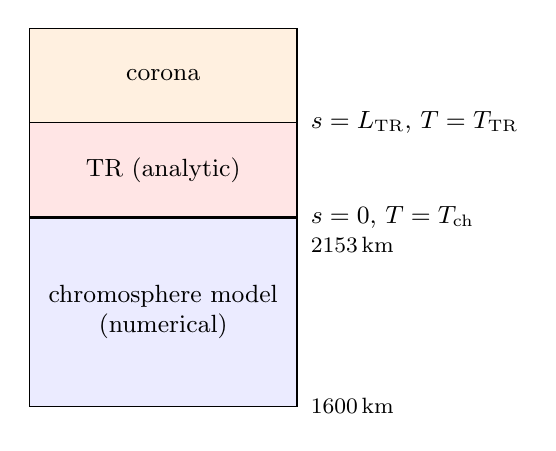
\begin{tikzpicture}[x=1cm,y=1cm,font=\small]
        \fill[orange!12] (0,3.6) rectangle (3.4,4.8);
        \fill[red!10]    (0,2.4) rectangle (3.4,3.6);
        \fill[blue!8]    (0,0)   rectangle (3.4,2.4);
        \draw (0,0) rectangle (3.4,4.8);
        \draw (0,3.6) -- (3.4,3.6);
        \draw[very thick] (0,2.4) -- (3.4,2.4);
        \node at (1.7,4.2) {corona};
        \node at (1.7,3.0) {TR (analytic)};
        \node[align=center] at (1.7,1.2) {chromosphere model\\(numerical)};
        \node[right] at (3.45,3.6) {$s=\LTR$, $T=\TTR$};
        \node[right] at (3.45,2.4) {$s=0$, $T=\Tch$};
        \node[right] at (3.45,2.05) {\footnotesize 2153\,km};
        \node[right] at (3.45,0)   {\footnotesize 1600\,km};
      \end{tikzpicture}
    \end{column}
    \begin{column}{0.46\textwidth}
      \begin{result}{Top boundary today (both fixed)}
        $\Tch = 22$\,kK,\quad $P = 0.0103$\,Pa
      \end{result}
      \begin{result}{Proposal}
        Keep $\Tch$; replace the fixed $P$ by $\PTR$ from a steady TR above $s=0$.
      \end{result}
      At $s=0$:
      \begin{itemize}
        \item chromosphere $\to$ TR: $\rho u$, $\qch$
        \item TR $\to$ chromosphere: $\PTR$
        \item given: $\TTR$, $\LTR$
      \end{itemize}
    \end{column}
  \end{columns}
\end{frame}

%----------------------------------------------------------------------
\begin{frame}{Reference case}
  \begin{estimate}{Numbers used in the estimates below}
    \centering
    \small
    \begin{tabular}{@{}l l l@{}}
      $\Tch$ & 22\,kK & today's top-boundary temperature \\
      $\PTR$ & 0.0103\,Pa & today's top-boundary pressure \\
      $\LTR$ & 1.5\,Mm & assumed \\
      $\TTR$ & 477\,kK & chosen: TR model gives 0.0103\,Pa at $\rho u=0$ \\
      $\rho u$ & $2.68\times10^{-10}$\,kg\,m$^{-2}$\,s$^{-1}$ & chromosphere model, top face, $t=4000$\,s \\
      $\qch$ & 0.53\,W\,m$^{-2}$ & chromosphere model, top face, $t=4000$\,s \\
      $u_{\rm ch}=\rho u/\rho_{\rm ch}$ & 9.5\,m\,s$^{-1}$ & TR-bottom velocity, $\rho_{\rm ch}=m_p\PTR/(2k_B\Tch)$ \\
      $u_{\rm TR}$ & 205\,m\,s$^{-1}$ & TR-top velocity, same with $\TTR$ (and $P\approx\PTR$) \\
      $g$ & 274\,m\,s$^{-2}$ & $GM_\odot/R_\odot^2$ \\
    \end{tabular}
  \end{estimate}
  {\small $^\dagger$\,Taken from the final TR solution ($q_{\rm TR}$, radiated power, integrals
  over $s$); used only to check, afterward, that the dropped terms are small.}

  \vspace{0.5em}
  {\small Boxes:\
  \colorbox{amber!25}{assumption}\
  \colorbox{estc!20}{estimate}\
  \colorbox{navy!15}{equation / result}\
  {\color{alertc}\textbf{$\Rightarrow$ conclusion}}}
\end{frame}

%----------------------------------------------------------------------
\begin{frame}{Equations along the field line ($0\le s\le\LTR$)}
  \begin{result}{Mass, momentum, energy}
    \vspace{-0.6em}
    \begin{align}
      &\frac{\partial\rho}{\partial t} + B\frac{\partial}{\partial s}\Big(\frac{\rho u}{B}\Big) = 0 \\
      &\frac{\partial(\rho u)}{\partial t} + B\frac{\partial}{\partial s}\Big(\frac{\rho u^2}{B}\Big)
        = -\frac{\partial P}{\partial s} - \rho g \\
      &\frac{\partial E}{\partial t} + B\frac{\partial}{\partial s}
        \left[\frac{(E+P)\,u - q}{B}\right]
        = -\rho u g + Q_{\rm heat} - N_eN_i\Lambda_R(T)
    \end{align}
  \end{result}
  \begin{result}{Pure hydrogen, ionization degree $x$}
    \[
      N_e = N_i = \frac{x\rho}{m_p},\quad P = (1+x)\frac{\rho k_BT}{m_p},\quad
      E = \frac{\rho u^2}{2} + \frac{P}{\gamma-1} + N_i\chi_{\rm H},\quad
      q = \kappa\frac{\partial T}{\partial s}
    \]
  \end{result}
  {\small $s$ upward from the interface; $q>0$: conductive flux toward the chromosphere;
  $\chi_{\rm H}=13.6$\,eV.}
\end{frame}

%----------------------------------------------------------------------
\begin{frame}{Step 1: steady}
  \begin{assume}{Assumption: $\partial/\partial t=0$}
    The TR relaxes faster than its inputs ($\rho u$, $\qch$) change.
  \end{assume}
  \begin{estimate}{Two timescales}
    \vspace{-0.5em}
    \begin{align*}
      \tau_{\rm TR} &= \frac{\text{thermal energy in TR}}{\text{heat conducted in}}
        = \frac{\tfrac32\PTR\LTR}{q_{\rm TR}^{\,\dagger}}
        = \frac{1.5\cdot0.0103\cdot1.5\times10^{6}}{163} \approx 140\ \text{s}\\
      \tau_{\rm drive} &= \frac{\rho u}{|\dd(\rho u)/\dd t|}
        = \frac{2.68\times10^{-10}}{1.65\times10^{-14}} \approx 1.6\times10^4\ \text{s}
    \end{align*}
    {\small $\dd(\rho u)/\dd t$: chromosphere model at $t=4000$\,s ($\rho u$ falls 3.1\,\% per 500\,s).}
  \end{estimate}
  \concl{$\tau_{\rm TR}/\tau_{\rm drive}\approx0.01$: time-derivative terms $\sim1\,\%$, drop.}
\end{frame}

%----------------------------------------------------------------------
\begin{frame}{Step 2: constant $B$}
  \begin{assume}{Assumption: $B=\text{const}$}
    Same as the chromosphere model.
  \end{assume}
  \begin{result}{Equations (1)--(3) after steps 1--2}
    \vspace{-0.6em}
    \begin{gather}
      \frac{\dd(\rho u)}{\dd s} = 0 \quad\Rightarrow\quad \rho u = \text{const} \\[0.2em]
      \frac{\dd}{\dd s}\big(P + \rho u^2\big) = -\rho g \\[0.2em]
      \frac{\dd}{\dd s}\left[\rho u\,\frac{E+P}{\rho} - q\right]
        = -\rho u g + Q_{\rm heat} - N_eN_i\Lambda_R(T)
    \end{gather}
  \end{result}
\end{frame}

%----------------------------------------------------------------------
\begin{frame}{Step 3: full ionization}
  \begin{assume}{Assumption: $x=1$}
    Saha at 22\,kK, 0.01\,Pa: $1-x\approx3\times10^{-9}$; smaller at higher $T$.
  \end{assume}
  \begin{result}{Closures with $x=1$}
    \[
      P = 2N_ik_BT,\quad \rho = m_pN_i,\quad \kappa = \kappa_0T^{5/2},\quad
      \frac{E+P}{\rho} = \frac{u^2}{2} + \kg\frac{k_BT}{m_p} + \frac{\chi_{\rm H}}{m_p}
    \]
  \end{result}
  Ionization term in (6):
  \[
    \frac{\dd}{\dd s}\left(\rho u\,\frac{\chi_{\rm H}}{m_p}\right) = 0
    \qquad\text{since } \rho u = \text{const}
  \]
  \concl{drops out exactly.}
\end{frame}

%----------------------------------------------------------------------
\begin{frame}{Step 4: energy equation, every term}
  \begin{result}{(6) integrated over the TR, all terms kept ($\gamma=5/3$, $\Delta T=\TTR-\Tch$)}
    \[
      q_{\rm TR} - \qch
      = \rho u\,\frac{5k_B\Delta T}{m_p}
      + \rho u\,\Delta\Big(\frac{u^2}{2}\Big)
      + \rho u\,g\,\LTR
      - \!\int\! Q_{\rm heat}\,\dd s
      + \!\int\! N_eN_i\Lambda_R\,\dd s
    \]
  \end{result}
  \begin{estimate}{Each term [W\,m$^{-2}$]}
    \centering
    \small
    \begin{tabular}{@{}l l r@{}}
      heat in minus out & $q_{\rm TR}^{\,\dagger} - \qch = 163 - 0.5$ & 162 \\
      heating the upflow & $2.68\times10^{-10}\cdot 5k_B(477-22)\,\text{kK}/m_p$ & 5.0 \\
      kinetic energy & $2.68\times10^{-10}\cdot(205^2-9.5^2)/2$ & $5.6\times10^{-6}$ \\
      gravity work & $2.68\times10^{-10}\cdot274\cdot1.5\times10^{6}$ & 0.11 \\
      heating in TR & step 6 & -- \\
      radiation$^\dagger$ & remainder & 157 \\
    \end{tabular}
  \end{estimate}
\end{frame}

%----------------------------------------------------------------------
\begin{frame}{Step 4: ratios of small to large terms}
  \begin{estimate}{Kinetic energy}
    \vspace{-0.5em}
    \begin{align*}
      \frac{\text{kinetic}}{\text{upflow heating}}
        &= \frac{m_p\,\Delta(u^2/2)}{5k_B\Delta T}
         = \frac{(205^2-9.5^2)/2}{1.88\times10^{10}}
         = 1.1\times10^{-6} \\
      \frac{\text{kinetic}}{\text{heat in}}
        &= \frac{\rho u\,\Delta(u^2/2)}{q_{\rm TR}-\qch}
         = \frac{5.6\times10^{-6}}{162}
         = 3.5\times10^{-8}
    \end{align*}
  \end{estimate}
  \begin{estimate}{Gravity work}
    \vspace{-0.5em}
    \begin{align*}
      \frac{\text{gravity work}}{\text{upflow heating}}
        &= \frac{m_p\,g\,\LTR}{5k_B\Delta T}
         = \frac{1.67\times10^{-27}\cdot274\cdot1.5\times10^{6}}{5\cdot1.38\times10^{-23}\cdot4.55\times10^{5}}
         = 0.022 \\
      \frac{\text{gravity work}}{\text{heat in}}
        &= \frac{\rho u\,g\,\LTR}{q_{\rm TR}-\qch}
         = \frac{0.11}{162}
         = 6.8\times10^{-4}
    \end{align*}
  \end{estimate}
  \concl{drop both: at most 2\,\% of the upflow heating, $<10^{-3}$ of the heat budget.}
\end{frame}

%----------------------------------------------------------------------
\begin{frame}{Step 5: momentum equation, every term}
  \begin{result}{(5) integrated over the TR}
    \[
      \Delta\big(P + \rho u^2\big) = -\int_0^{\LTR}\rho g\,\dd s
    \]
  \end{result}
  \begin{estimate}{Dynamic pressure vs.\ pressure (with $P\approx\PTR$)}
    \[
      \frac{\rho u^2}{P}:\quad
      \text{bottom } \frac{2.8\times10^{-11}\cdot 9.5^2}{0.0103} = 2.5\times10^{-7},\quad
      \text{top } \frac{1.3\times10^{-12}\cdot 205^2}{0.0103} = 5\times10^{-6}
    \]
  \end{estimate}
  \begin{estimate}{Gravity: $\dd\ln P/\dd s = -1/H$,\ $H = 2k_BT/(m_pg)$, along the TR profile$^\dagger$}
    \[
      H(22\,\text{kK}) = 1.3\,\text{Mm},\quad H(477\,\text{kK}) = 29\,\text{Mm};\qquad
      \Delta\ln P = \int_0^{\LTR}\frac{\dd s}{H} \approx 0.086
    \]
  \end{estimate}
  \concl{drop both (gravity: 8\,\%, the largest dropped term) $\Rightarrow$ $P=\PTR$ in the TR.}
\end{frame}

%----------------------------------------------------------------------
\begin{frame}{Step 6 and the simplified equations}
  \begin{assume}{Assumption: $Q_{\rm heat}=0$ in the TR}
    Heat is deposited above the TR.
  \end{assume}
  \begin{result}{Equations (4)--(6) after steps 3--6}
    \vspace{-0.6em}
    \begin{gather}
      \rho u = \text{const},\qquad P = \PTR,\qquad N_e=N_i=\frac{\PTR}{2k_BT},\qquad
      q = \kappa_0T^{5/2}\frac{\dd T}{\dd s} \\[0.2em]
      \frac{\dd}{\dd s}\left(\rho u\,\kg\frac{k_BT}{m_p} - q\right) = -N_eN_i\Lambda_R(T)
    \end{gather}
  \end{result}
  Integrated: heat in $=$ heat out $+$ upflow heating $+$ radiation
  \[ 163 = 0.5 + 5.0 + 157\ \ \text{W\,m}^{-2} \]
\end{frame}

%----------------------------------------------------------------------
\begin{frame}{Step 7: change variable $s\to T$}
  $q>0$ $\Rightarrow$ $T$ increases with $s$:
  \[
    \frac{\dd T}{\dd s} = \frac{q}{\kappa_0T^{5/2}},\qquad
    \frac{\dd}{\dd s} = \frac{q}{\kappa_0T^{5/2}}\frac{\dd}{\dd T}
  \]
  Substitute into (8), multiply by $\kappa_0T^{5/2}$:
  \vspace{-0.3em}
  \[
    q\left(\kg\frac{k_B\rho u}{m_p} - \frac{\dd q}{\dd T}\right)
    = -\kappa_0T^{5/2}\,\frac{\PTR^2}{4k_B^2T^2}\,\Lambda_R(T)
  \]
  \begin{result}{With $2q\,\dd q/\dd T = \dd(q^2)/\dd T$}
    \begin{equation}
      \frac{\dd(q^2)}{\dd T}
      = \underbrace{\frac{4\gamma}{\gamma-1}\frac{k_B\rho u}{m_p}\,q}_{\text{heats the upflow}}
      + \underbrace{\frac{\kappa_0\PTR^2}{2k_B^2}\sqrt{T}\,\Lambda_R(T)}_{\text{radiation}},
      \qquad q(\Tch)=\qch
      \label{eq:q2}
    \end{equation}
  \end{result}
\end{frame}

%----------------------------------------------------------------------
\begin{frame}{Result}
  \begin{result}{Thickness, from $\dd s = \kappa_0T^{5/2}\,\dd T/q$:\ $\PTR$ is the root}
    \begin{equation}
      \int_{\Tch}^{\TTR}\frac{\kappa_0T^{5/2}}{q(T;\,\PTR,\rho u,\qch)}\,\dd T = \LTR,
      \qquad q\ \text{from \eqref{eq:q2}}
    \end{equation}
  \end{result}
  \begin{itemize}
    \item Larger $\PTR$ $\Rightarrow$ larger $q$ $\Rightarrow$ smaller integral
          $\Rightarrow$ unique root.
    \item Needs $q>0$ up to $\TTR$; strong downflow has no solution
          (limit $u_{\rm ch}\in[-40,100]$\,m\,s$^{-1}$).
  \end{itemize}
  \begin{result}{No flow ($\rho u=0$, $\qch=0$): $q = \tfrac12\PTR\,U_{\rm heat}(T)$}
    \[
      \frac{\PTR}{2} = \frac{1}{\LTR}\int_{\Tch}^{\TTR}\frac{\kappa_0T^{5/2}}{U_{\rm heat}(T)}\,\dd T,
      \qquad
      U_{\rm heat}(T) = \sqrt{\frac{2}{k_B^2}\int_{\Tch}^{T}\kappa_0T'^{1/2}\Lambda_R(T')\,\dd T'}
    \]
  \end{result}
\end{frame}

%----------------------------------------------------------------------
\begin{frame}{Numbers}
  \begin{estimate}{$\PTR$ and its flow correction
      ($\Tch=22$\,kK, $\LTR=1.5$\,Mm, $\qch=0.527$\,W\,m$^{-2}$, CHIANTI 8.0)}
    \centering
    \begin{tabular}{@{}l r r r r r r@{}}
      & $\PTR$ [Pa] & \multicolumn{5}{c}{change of $\PTR$ for $u_{\rm ch}$ [m\,s$^{-1}$]} \\
      \cmidrule(l){3-7}
      $\TTR$ & $\rho u=0$ & $-40$ & $-10$ & $+10$ & $+30$ & $+100$ \\
      \midrule
      300\,kK  & 0.0029 & $+5.3\,\%$ & $+1.3\,\%$ & $-1.3\,\%$ & $-3.7\,\%$  & $-11.9\,\%$ \\
      477\,kK  & 0.0103 & $+6.8\,\%$ & $+1.6\,\%$ & $-1.6\,\%$ & $-4.7\,\%$  & $-14.5\,\%$ \\
      1\,MK    & 0.083  & $+9.6\,\%$ & $+2.3\,\%$ & $-2.2\,\%$ & $-6.4\,\%$  & $-19.3\,\%$ \\
    \end{tabular}
  \end{estimate}
  \begin{itemize}
    \item Check of the reference case: $\TTR=477$\,kK gives 0.0103\,Pa at $\rho u=0$.
    \item Present evaporation, $\rho u=2.68\times10^{-10}$\,kg\,m$^{-2}$\,s$^{-1}$
          ($u_{\rm ch}\approx9.6$\,m\,s$^{-1}$ at the lowered $\PTR$):
          \alert{$\PTR$ lower by 1.5\,\%.}
  \end{itemize}
\end{frame}

%----------------------------------------------------------------------
\begin{frame}{Boundary condition}
  \begin{result}{Ghost cell above $s=0$, each step}
    \[
      P = \PTR,\qquad T = \Tch,\qquad \rho = \frac{m_p\PTR}{2k_B\Tch},\qquad u\ \text{as now}
    \]
  \end{result}
  \centering
  \begin{tabular}{@{}l l@{}}
    \toprule
    $\Tch$ & 22\,kK, fixed \\
    $\TTR$, $\LTR$ & given (477\,kK, 1.5\,Mm) \\
    $\rho u$ & mass flux through the top face, previous step \\
    $\qch$ & conductive flux at the top face, previous step \\
    $\kappa_0$ & $9.2048\times10^{-12}$\,W\,m$^{-1}$\,K$^{-7/2}$ (same as chromosphere model) \\
    \bottomrule
  \end{tabular}
\end{frame}

\end{document}
